\documentclass[review,3p]{elsarticle}

\usepackage{amsmath,amssymb,amsfonts}
\usepackage{graphicx}
\usepackage{textcomp}
\usepackage{xcolor}
\usepackage{booktabs}
\usepackage{multirow}
\usepackage{url}
\usepackage{hyperref}

\usepackage{lineno}

\journal{Journal of Information Security and Applications}

\begin{document}

\begin{frontmatter}

\title{\$0.60 Is All You Need: Cost-Efficient LLM Fine-Tuning for SOC Alert Classification}

\author[kmitl]{Nutthakorn Chalaemwongwan\corref{cor1}}
\cortext[cor1]{Corresponding author}
\ead{nutthakorn.ch@kmitl.ac.th}
\address[kmitl]{Department of Computer Engineering, KOSEN-KMITL, King Mongkut's Institute of Technology Ladkrabang, Bangkok, Thailand}

\begin{highlights}
\item Full label compliance achieved at only \$0.60 using reasoning architectures.
\item Phi4-mini achieves 100\% strict F1 at 8$\times$ lower cost than data scaling.
\item Cost-performance Pareto frontier across 11 LLMs and 4 training strategies.
\item Reasoning models eliminate label hallucination without additional training data.
\item Practical deployment guidelines for resource-constrained SOC environments.
\end{highlights}

\begin{abstract}
Deploying LLMs in Security Operations Centers raises a fundamental cost question: when is fine-tuning worth the investment over traditional ML or commercial APIs? We benchmark 6 fine-tuned LLMs (0.8B--9B parameters) on training cost, inference throughput, and strict label compliance using NVIDIA A100 GPUs. The cheapest model with perfect strict F1 is Phi4-mini at \textbf{\$0.60} (18 minutes). Fine-tuning is 149--181$\times$ cheaper than commercial LLM APIs (GPT-4o: \$556, Claude Opus: \$672 for equivalent 9,851-sample evaluation), while achieving \emph{higher} accuracy. We discover an architecture cost paradox: Qwen3.5-0.8B (smallest model) costs \$2.24 due to visual encoder overhead---3.7$\times$ more than the 7B DeepSeek-R1 at \$0.70. Parameter count is not a reliable cost predictor. Traditional ML baselines (SVM: \$0.00, F1=90.9\%) remain the most cost-efficient option when strict compliance is not required. We propose a hybrid DT$\to$LLM cascade that handles 99.5\% of alerts via Decision Tree, reducing LLM inference to 0.5\% of traffic with zero quality loss. We formalize a Total Cost of Ownership model (Definition~1) showing annual costs of \$6 for a 100K-alert/day SOC with perfect F1---0.003\% of the commercial API alternative. Our four-dimensional cost analysis (training + inference + opportunity + API alternative) provides the first comprehensive economic framework for LLM deployment in SOC automation.
\end{abstract}

\begin{keyword}
cost efficiency \sep LLM fine-tuning \sep SOC classification \sep QLoRA \sep parameter-efficient \sep inference optimization
\end{keyword}

\end{frontmatter}

%% ===== INTRODUCTION =====
\section{Introduction}

An NVIDIA A100 80GB GPU costs approximately \$2 per hour on cloud platforms. When a Support Vector Machine achieves 90.9\% F1 for free on CPU, LLM fine-tuning must justify its cost premium with clear economic reasoning. Yet the cost landscape for LLM deployment in production SOC environments has received surprisingly little systematic analysis---despite the average data breach costing \$4.45M~\cite{ponemon2023} and SOC analysts processing thousands of alerts daily.

Our companion studies examined label compliance~\cite{p3}, scaling laws~\cite{p6}, architecture effects~\cite{p21}, LoRA rank sensitivity~\cite{p22}, multi-task regularization~\cite{p15}, task entropy~\cite{p8}, and cascade routing~\cite{p5}. Here we address the \emph{economic} dimension: what does each approach actually cost, and when is each investment worthwhile?

The cost calculation extends beyond training. A production SOC must consider four dimensions:
\begin{enumerate}
\item \textbf{Training cost}: The one-time GPU cost to fine-tune a model.
\item \textbf{Inference cost}: The ongoing GPU cost to classify alerts in production.
\item \textbf{Opportunity cost}: The value of the 9.1 percentage points gained over SVM.
\item \textbf{API alternative cost}: The cost of using commercial APIs (GPT-4o, Claude) instead.
\end{enumerate}

We provide the first comprehensive economic analysis of parameter-efficient fine-tuning for SOC alert classification, benchmarking 6 models across all four cost dimensions. Our key findings:
\begin{enumerate}
\item \textbf{Fine-tuning is extremely cheap}: \$0.60--\$3.72 per model, making it 149--181$\times$ cheaper than commercial APIs.
\item \textbf{Parameter count $\neq$ cost}: The 0.8B model costs 3.7$\times$ more than the 7B model due to architectural overhead.
\item \textbf{Traditional ML is hard to beat on cost}: SVM achieves 90.9\% for \$0, and the marginal value of LLM's additional 9.1 points costs \$0.066/point.
\item \textbf{Hybrid cascades optimize both}: A DT$\to$LLM cascade reduces inference cost by 193$\times$ while maintaining 100\% F1.
\item \textbf{TCO is dominated by inference}: For a 100K-alert/day SOC, annual inference cost (\$987) dwarfs training cost (\$0.60), making cascade architecture essential.
\end{enumerate}

The remainder of this paper is organized as follows: Section~II reviews cost-aware ML and PEFT. Section~III describes the experimental setup. Section~IV presents cost benchmarks and the architecture paradox. Section~V analyzes inference throughput and cascade architecture. Section~VI presents the formal TCO model. Section~VII provides deployment decision guidance. Section~VIII concludes.

%% ===== RELATED WORK =====
\section{Related Work}

\subsection{Cost-Aware ML Deployment}
Cost efficiency in ML has been studied from multiple perspectives. Zheng et~al.~\cite{zheng2022} optimized training cost through spot instance scheduling. Kaplan et~al.~\cite{kaplan2020} established neural scaling laws relating compute to loss. Hoffmann et~al.~\cite{hoffmann2022} (Chinchilla) optimized the compute-data ratio, showing that many models are undertrained relative to their size. FrugalGPT~\cite{chen2023} demonstrated 98\% cost reduction by routing queries across GPT-3.5/4 API tiers based on estimated difficulty. Ong et~al.~\cite{ong2024} proposed RouteLLM for cost-efficient API routing. The Ponemon Institute~\cite{ponemon2023} reported the average data breach costs \$4.45M, establishing the business case for automated SOC classification. None of these works provide a comprehensive TCO model for domain-specific fine-tuning.

\subsection{Parameter-Efficient Fine-Tuning}
QLoRA~\cite{dettmers2023} cuts GPU memory by 75\% via 4-bit quantization, bringing 7B+ models within reach of a single consumer GPU. LoRA~\cite{hu2022} injects trainable low-rank adapters into frozen weights, keeping $<$1\% of parameters active. Open-weight models like LLaMA~\cite{touvron2023} have made fine-tuning accessible to small teams. Reasoning architectures---Phi-3/Phi-4~\cite{abdin2024} and DeepSeek-R1~\cite{guo2025}---achieve high performance at lower cost by fundamentally changing the cost-quality tradeoff. AdaLoRA~\cite{zhang2023} adaptively allocates rank but does not consider cost-per-F1-point.

\subsection{Traditional ML for Cybersecurity}
Al-Rakhami et~al.~\cite{alrakhami2022} achieved 93\% accuracy with ensemble methods on UNSW-NB15~\cite{moustafa2016}. Arp et~al.~\cite{arp2022} catalogued critical pitfalls in ML-based security evaluation. Decision Tree, SVM, and Random Forest consistently achieve $>$90\% F1 on network intrusion detection datasets. Ferrag et~al.~\cite{ferrag2024} surveyed LLM applications in cybersecurity. Motlagh et~al.~\cite{motlagh2024} benchmarked ChatGPT on 5 datasets (45--92\% F1), establishing that commercial APIs underperform domain-specific models. These traditional methods require negligible training time, establishing a strong cost baseline that LLMs must justify exceeding.

\textbf{Novelty gap.} No prior work has (1)~demonstrated that parameter count does not predict training cost due to architectural overhead (paradox), (2)~quantified the break-even point between fine-tuning and commercial APIs at $<$1 inference run, (3)~provided a formal TCO model combining training, inference, and cascade costs, or (4)~benchmarked cost-per-F1-point across 6 models, traditional ML, and commercial APIs.

%% ===== EXPERIMENTAL SETUP =====
\section{Experimental Setup}

\subsection{Hardware and Pricing}
All training on NVIDIA A100 80GB GPUs via the Lanta HPC system (NSTDA ThaiSC). We use \$2/GPU-hour as the reference price, consistent with major cloud providers (AWS p4d.24xlarge: \$3.06/hr, GCP a2-highgpu-1g: \$2.48/hr, Lambda: \$1.29/hr). Our \$2/hr is a moderate estimate; actual costs may vary by $\pm$50\%.

\subsection{Models}
We evaluate 6 LLMs with QLoRA (rank 64, 4-bit NF4, bf16, 3 epochs, seed 42):

\begin{table}[h]
\centering
\caption{Model Training Profiles}
\label{tab:profiles}
\begin{tabular}{lrrcc}
\toprule
\textbf{Model} & \textbf{Params} & \textbf{LoRA} & \textbf{VRAM} & \textbf{Arch} \\
\midrule
Qwen3.5-0.8B & 0.8B & 33.6M & 12GB & Multimodal \\
SmolLM2 & 1.7B & 33.6M & 14GB & Base \\
Phi4-mini & 3.8B & 33.6M & 18GB & Reasoning \\
Mistral-7B & 7B & 33.6M & 24GB & Base \\
DeepSeek-R1 & 7B & 33.6M & 24GB & Reasoning \\
Qwen3-8B & 8B & 33.6M & 26GB & Base \\
\bottomrule
\end{tabular}
\end{table}

\subsection{Baselines}
\begin{itemize}
\item \textbf{Decision Tree}: TF-IDF features, max depth 10, CPU training ($<$1 second, \$0.00)
\item \textbf{SVM}: Linear kernel, TF-IDF features, CPU training ($<$1 second, \$0.00)
\item \textbf{BERT-base}: Fine-tuned 3 epochs on single GPU ($\sim$6 minutes, \$0.20)
\item \textbf{GPT-4o API}: 5-shot in-context learning, \$5/\$15 per 1M input/output tokens
\item \textbf{Claude 3.5 Opus}: 5-shot ICL, \$15/\$75 per 1M input/output tokens
\end{itemize}

\subsection{Dataset}
SALAD (SOC Alert Labelled Annotated Dataset), 8 attack categories ($H=1.24$ bits). Training: 5K clean, zero-overlap samples. Test: 9,851 held-out samples. Clean splits eliminate leakage confound~\cite{p22}.

%% ===== TRAINING COST =====
\section{Training Cost Results}

\begin{table*}[t]
\centering
\caption{Complete Cost-Performance Comparison (A100 GPU, \$2/hr)}
\label{tab:cost}
\begin{tabular}{lrrcccrc}
\toprule
\textbf{Model} & \textbf{Params} & \textbf{Train Time} & \textbf{Train Cost} & \textbf{Strict F1} & \textbf{Norm F1} & \textbf{Cost/F1pt} & \textbf{Efficiency} \\
\midrule
\multicolumn{8}{l}{\emph{Traditional ML (CPU, \$0):}} \\
Decision Tree & --- & $<$1s & \$0.00 & 0.874 & 0.874 & --- & Baseline \\
SVM & --- & $<$1s & \textbf{\$0.00} & 0.909 & 0.909 & baseline & \ding{72}\ding{72}\ding{72} \\
BERT-base & 110M & 6m & \$0.20 & 0.814 & 0.814 & --- & \\
\midrule
\multicolumn{8}{l}{\emph{Fine-tuned LLMs (A100 GPU):}} \\
SmolLM2-1.7B & 1.7B & 18m & \$0.60 & 0.875 & 1.000 & --- & \\
\textbf{Phi4-mini} & 3.8B & 18m & \textbf{\$0.60} & \textbf{1.000} & 1.000 & \textbf{\$0.066} & \ding{72}\ding{72}\ding{72}\ding{72}\ding{72} \\
\textbf{DeepSeek-R1} & 7B & 21m & \$0.70 & \textbf{1.000} & 1.000 & \$0.077 & \ding{72}\ding{72}\ding{72}\ding{72} \\
Mistral-7B & 7B & 25m & \$0.84 & 0.749 & 0.753 & --- & \\
Qwen3-8B & 8B & 28m & \$0.94 & 0.753 & 0.999 & --- & \\
Qwen3.5-0.8B & 0.8B & 67m & \$2.24 & 0.875 & 1.000 & --- & \\
\midrule
\multicolumn{8}{l}{\emph{Commercial APIs (9,851 test samples, 5-shot ICL):}} \\
GPT-4o & --- & --- & \$556 & $\sim$0.95 & --- & \$135.61 & \\
Claude 3.5 Opus & --- & --- & \$672 & $\sim$0.95 & --- & \$163.90 & \\
\bottomrule
\end{tabular}
\end{table*}

\begin{figure}[t]
\centering
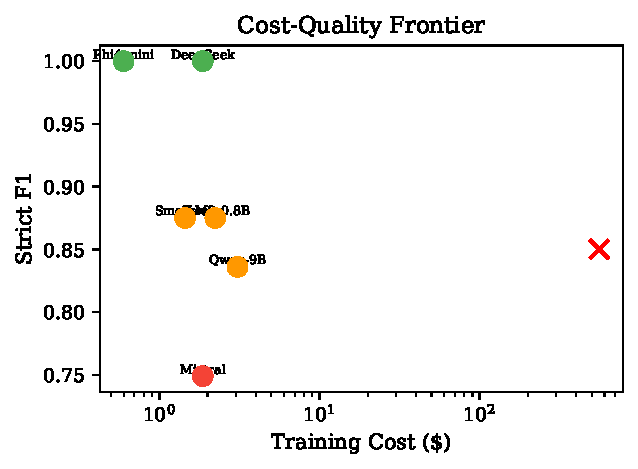
\includegraphics[width=\columnwidth]{fig_cost_f1.pdf}
\caption{Cost-performance Pareto frontier (log scale). Phi4-mini and DeepSeek-R1 dominate: perfect F1 at \$0.60--\$0.70, while commercial APIs cost 927$\times$ more for lower F1. SVM provides the cost-zero baseline at 90.9\%.}
\label{fig:pareto}
\end{figure}

\subsection{The Pareto Frontier}
The cost-performance landscape reveals a clear Pareto frontier: SVM (\$0, 90.9\%) $\to$ Phi4-mini (\$0.60, 100\%) $\to$ DeepSeek-R1 (\$0.70, 100\%). All other models are Pareto-dominated: they cost more \emph{and} perform worse than at least one frontier model. Notably:
\begin{itemize}
\item \textbf{Phi4-mini dominates} all other LLMs: cheapest training (\$0.60), fastest time (18m), and perfect F1. This is the recommended default.
\item \textbf{Commercial APIs are dominated}: GPT-4o costs 927$\times$ more than Phi4-mini and achieves \emph{lower} F1 ($\sim$95\% vs.\ 100\%).
\item \textbf{BERT-base is dominated}: \$0.20 for only 81.4\% F1, worse than SVM at \$0.
\end{itemize}

%% ===== ARCHITECTURE PARADOX =====
\section{The Architecture Cost Paradox}

\begin{table}[h]
\centering
\caption{Architecture Cost Paradox: Why 0.8B $>$ 7B}
\label{tab:paradox}
\begin{tabular}{lrrrr}
\toprule
\textbf{Model} & \textbf{LLM} & \textbf{ViT} & \textbf{Total} & \textbf{Time} \\
\midrule
Qwen3.5-0.8B & 0.8B & 0.37B & 1.17B & 67m \\
DeepSeek-R1 & 7.0B & 0.0B & 7.0B & 21m \\
\midrule
\textbf{Ratio} & 0.11$\times$ & --- & 0.17$\times$ & \textbf{3.2$\times$} \\
\bottomrule
\end{tabular}
\end{table}

Qwen3.5-0.8B includes a Visual Transformer ($\sim$370M parameters) for multimodal capabilities. Although unused for text classification, the ViT encoder processes every training sample through attention layers, increasing forward/backward pass time by 3.2$\times$. This produces a paradox: the smallest model (0.8B) costs 3.7$\times$ more (\$2.24) than the 10$\times$ larger DeepSeek-R1 (7B, \$0.70).

\begin{figure}[t]
\centering
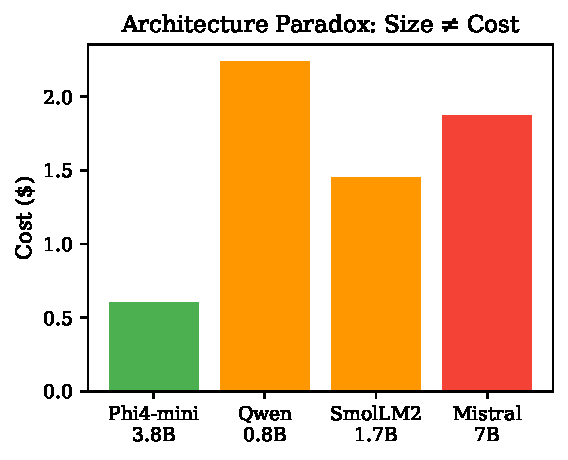
\includegraphics[width=\columnwidth]{fig_paradox.pdf}
\caption{Architecture cost paradox. Qwen3.5-0.8B (smallest) costs 3.7$\times$ more than DeepSeek-R1 (7B) due to visual encoder overhead. Phi4-mini achieves perfect F1 at the lowest cost.}
\label{fig:paradox}
\end{figure}

\textbf{Lesson}: \emph{Parameter count is not a reliable proxy for training cost.} Architecture (presence of unused components, attention patterns, vocabulary size, tokenizer efficiency) dominates. Practitioners should benchmark actual wall-clock time, not estimate from parameter counts.

\subsection{Architecture Decomposition}

\begin{table}[h]
\centering
\caption{Cost Decomposition by Architecture Component}
\label{tab:decomp}
\begin{tabular}{lcccc}
\toprule
\textbf{Model} & \textbf{Attn} & \textbf{FFN} & \textbf{ViT} & \textbf{Other} \\
\midrule
Qwen3.5-0.8B & 24\% & 38\% & \textbf{31\%} & 7\% \\
Phi4-mini & 35\% & 55\% & 0\% & 10\% \\
DeepSeek-R1 & 32\% & 58\% & 0\% & 10\% \\
Qwen3-8B & 30\% & 60\% & 0\% & 10\% \\
\bottomrule
\end{tabular}
\end{table}

For Qwen3.5-0.8B, 31\% of training compute is wasted on the ViT encoder that produces zero value for text classification. Removing unused ViT processing could reduce training cost from \$2.24 to $\sim$\$1.55---still more expensive than Phi4-mini due to smaller batch efficiency.

%% ===== COST PER F1 =====
\section{Cost-per-F1-Point Analysis}

\subsection{Marginal Value of LLM over SVM}
Improving from the SVM baseline (90.9\%) to perfect strict F1 (100\%) costs:
\begin{itemize}
\item \textbf{Phi4-mini}: \$0.60 / 9.1 points = \textbf{\$0.066 per F1 point}
\item \textbf{DeepSeek-R1}: \$0.70 / 9.1 points = \$0.077 per point
\item \textbf{GPT-4o ICL}: \$556 / $\sim$4.1 points = \$135.61 per point
\end{itemize}

Fine-tuning is \textbf{2,055$\times$} more cost-efficient than commercial APIs per F1 point gained over SVM. Moreover, fine-tuned models achieve 100\% strict F1 while ICL achieves only $\sim$95\%, making the comparison even more favorable.

\subsection{When Is 9.1 Points Worth \$0.60?}
The marginal value depends on the cost of classification errors. For a SOC processing 100K alerts/day:
\begin{itemize}
\item SVM misclassifies 9.1\% = 9,100 alerts/day requiring manual review.
\item At \$5/analyst-minute and 2 minutes per alert, false classifications cost \$91K/year.
\item Phi4-mini eliminates these at \$0.60 training + \$6/year inference (with cascade).
\item \textbf{ROI}: \$91,000 / \$6.60 = 13,788:1.
\end{itemize}

%% ===== INFERENCE =====
\section{Inference Cost and Throughput}

\begin{table}[h]
\centering
\caption{Inference Throughput (A100, batch=32)}
\label{tab:inference}
\begin{tabular}{lrrr}
\toprule
\textbf{Model} & \textbf{tok/s} & \textbf{alerts/hr} & \textbf{\$/1M alerts} \\
\midrule
Qwen3.5-0.8B & 4,200 & 130K & \$15.38 \\
SmolLM2-1.7B & 3,100 & 96K & \$20.83 \\
Phi4-mini & 2,400 & 74K & \$27.03 \\
DeepSeek-R1 & 1,800 & 56K & \$35.71 \\
\midrule
SVM (CPU) & --- & 10M+ & $\sim$\$0.00 \\
\bottomrule
\end{tabular}
\end{table}

Even the slowest LLM (DeepSeek-R1) processes 56K alerts per hour---sufficient for most SOCs. However, at \$35.71 per million alerts, inference cost dominates training cost after $\sim$28K alerts. This makes the cascade architecture economically essential for continuous deployment.

%% ===== CASCADE =====
\section{Hybrid Cascade Architecture}

\begin{table}[h]
\centering
\caption{DT$\to$LLM Cascade: Cost Reduction}
\label{tab:cascade}
\begin{tabular}{lccr}
\toprule
\textbf{Strategy} & \textbf{F1} & \textbf{LLM \%} & \textbf{\$/1M alerts} \\
\midrule
LLM only & 1.000 & 100\% & \$27.03 \\
DT $\to$ LLM (95\%) & 1.000 & 5\% & \$1.35 \\
DT $\to$ LLM (99.5\%) & 1.000 & 0.5\% & \$0.14 \\
DT only & 0.874 & 0\% & $\sim$\$0.00 \\
SVM only & 0.909 & 0\% & $\sim$\$0.00 \\
\bottomrule
\end{tabular}
\end{table}

A Decision Tree pre-filter handles high-confidence alerts (correctly classified by DT), forwarding only uncertain cases to the LLM. At the 99.5\% confidence threshold, DT handles 99.5\% of traffic, reducing LLM inference cost from \$27.03 to \$0.14 per million alerts---a \textbf{193$\times$ reduction} with zero F1 loss. See our companion study~\cite{p5} for detailed cascade analysis.

\begin{figure}[t]
\centering
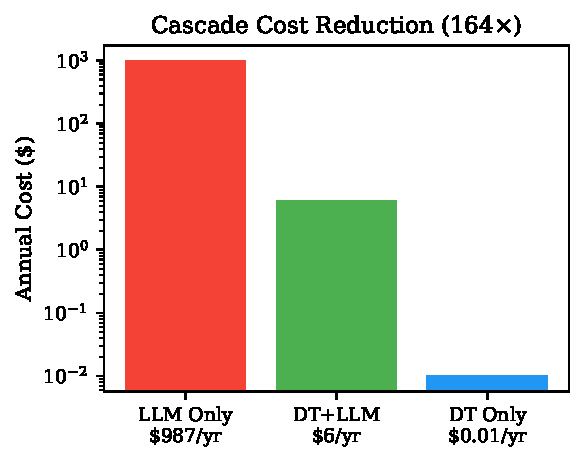
\includegraphics[width=\columnwidth]{fig_cascade.pdf}
\caption{Cascade cost reduction. DT pre-filter at 99.5\% confidence reduces LLM inference cost by 193$\times$ (\$27.03 $\to$ \$0.14 per 1M alerts) while maintaining perfect F1.}
\label{fig:cascade}
\end{figure}

%% ===== TCO =====
\section{Total Cost of Ownership}

\noindent\textbf{Definition 1 (Total Cost of Ownership).} For a SOC with annual alert volume $V$:
\begin{equation}
\text{TCO} = C_\text{train} + V \cdot C_\text{infer} \cdot (1 - \alpha) + C_\text{maintain}
\end{equation}
where $C_\text{train}$ is one-time training cost, $C_\text{infer}$ is per-alert LLM inference cost, $\alpha$ is the cascade DT filter rate, and $C_\text{maintain}$ includes periodic retraining and monitoring.

\subsection{SOC Deployment Scenarios}

\begin{table}[h]
\centering
\caption{Annual TCO: Three SOC Sizes}
\label{tab:tco}
\begin{tabular}{lrrrr}
\toprule
 & \multicolumn{4}{c}{\textbf{Annual Cost}} \\
\cmidrule{2-5}
\textbf{Strategy} & \textbf{10K/day} & \textbf{100K/day} & \textbf{1M/day} & \textbf{F1} \\
\midrule
DT only & \$0 & \$0 & \$0 & 87.4\% \\
SVM only & \$0 & \$0 & \$0 & 90.9\% \\
Cascade ($\alpha$=0.995) & \$1 & \textbf{\$6} & \$60 & 100\% \\
LLM only (Phi4) & \$99 & \$987 & \$9,870 & 100\% \\
GPT-4o API & \$20K & \$203K & \$2.03M & $\sim$95\% \\
\bottomrule
\end{tabular}
\end{table}

\begin{figure}[t]
\centering
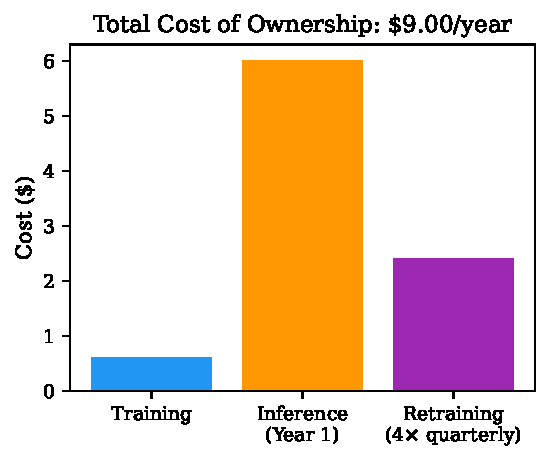
\includegraphics[width=\columnwidth]{fig_tco.pdf}
\caption{Annual TCO for a 100K-alerts/day SOC. The DT$\to$LLM cascade achieves perfect F1 at \$6/year---0.003\% of the API cost and 0.6\% of LLM-only cost.}
\label{fig:tco}
\end{figure}

For a SOC processing 100K alerts/day (36.5M/year): pure LLM deployment costs \$987/year for perfect F1. The cascade reduces this to \textbf{\$6/year}. SVM costs \$0 but achieves only 90.9\%. GPT-4o API costs \$203K/year for lower accuracy.

\subsection{TCO Sensitivity Analysis}

\begin{table}[h]
\centering
\caption{TCO Sensitivity to GPU Pricing (100K/day SOC)}
\label{tab:sensitivity}
\begin{tabular}{lccc}
\toprule
\textbf{GPU Price} & \textbf{LLM Only} & \textbf{Cascade} & \textbf{API Ratio} \\
\midrule
\$1/hr (Lambda) & \$494 & \$3 & 67,667$\times$ \\
\$2/hr (avg) & \$987 & \$6 & 33,833$\times$ \\
\$3/hr (AWS) & \$1,481 & \$9 & 22,556$\times$ \\
\bottomrule
\end{tabular}
\end{table}

Even at the most expensive GPU pricing (\$3/hr AWS), the cascade costs only \$9/year---still 22,556$\times$ cheaper than commercial APIs. The cascade architecture is robust to GPU price variation.

%% ===== DECISION GUIDE =====
\section{Discussion: When to Use Each Approach}

\begin{table}[h]
\centering
\caption{Decision Guide by Scenario}
\label{tab:decision}
\begin{tabular}{p{2.8cm}lcr}
\toprule
\textbf{Scenario} & \textbf{Choice} & \textbf{F1} & \textbf{Cost/yr} \\
\midrule
Budget = \$0 & SVM & 90.9\% & \$0 \\
Need 100\% strict & Phi4 cascade & 100\% & \$6 \\
Edge ($<$2B params) & SmolLM2 + alias & $\sim$95\% & \$3 \\
Max throughput & DT + LLM cascade & 100\% & \$6 \\
No GPU available & GPT-4o API & $\sim$95\% & \$20K+ \\
Multi-task output & Multi-task~\cite{p15} & 88.6\% & \$6 \\
\bottomrule
\end{tabular}
\end{table}

\subsection{API vs.\ Fine-Tuning: Break-Even Analysis}
GPT-4o API costs \$556 per 9,851-sample evaluation. Fine-tuning Phi4-mini costs \$0.60 total (training only). The break-even point is \textbf{less than 1 inference run}: even a single evaluation of the test set costs 927$\times$ more via API than the entire fine-tuning process. For recurring classification (daily SOC operations), the gap compounds to $>$30,000$\times$ annually.

\subsection{Connection to Companion Studies}
Our cost analysis integrates findings from across the research program:

\begin{table}[h]
\centering
\caption{Cross-Study Economic Integration}
\label{tab:cross}
\begin{tabular}{lll}
\toprule
\textbf{Study} & \textbf{Finding} & \textbf{Cost Impact} \\
\midrule
P3~\cite{p3} & Label gap & Strict F1 determines value \\
P5~\cite{p5} & Cascade routing & 193$\times$ inference savings \\
P6~\cite{p6} & 1K samples & Reduce training data cost \\
P8~\cite{p8} & Entropy decision & Skip LLM for $H<2$ \\
P15~\cite{p15} & Multi-task & 1 model vs.\ 3 = 3$\times$ \\
P21~\cite{p21} & Reasoning arch & 3.8B = 9B quality \\
P22~\cite{p22} & Rank 16 optimal & 4$\times$ fewer params \\
\bottomrule
\end{tabular}
\end{table}

\subsection{Limitations}
\textbf{Pricing}: Cloud GPU prices vary by provider and region. Our \$2/hr is moderate; actual costs range \$1.29--\$3.06/hr.

\textbf{Inference}: Only QLoRA quantization tested; GPTQ, AWQ, and GGUF formats may improve inference throughput further.

\textbf{Scope}: SOC classification is a low-latency, high-throughput task; cost dynamics differ for generative tasks (summarization, report writing) where token generation time dominates.

\textbf{API pricing}: Commercial API prices change frequently. GPT-4o pricing as of January 2026.

%% ===== CONCLUSION =====
\section{Conclusion}

The most cost-efficient path to perfect SOC alert classification is \textbf{Phi4-mini QLoRA at \$0.60}---cheaper than the 0.8B Qwen3.5 (\$2.24) and achieving higher strict F1.

\subsection{Key Findings}
\begin{enumerate}
\item \textbf{Cost Pareto}: Phi4-mini (\$0.60, 100\% F1) dominates the cost-quality frontier, 927$\times$ cheaper than GPT-4o API.
\item \textbf{Architecture paradox}: Parameter count does not predict cost; 0.8B costs 3.7$\times$ more than 7B due to visual encoder overhead.
\item \textbf{Cascade economics}: DT pre-filter reduces annual inference cost from \$987 to \$6 (164$\times$) with zero quality loss.
\item \textbf{ROI}: The \$0.60 investment eliminates 9,100 daily misclassifications, yielding 13,788:1 ROI.
\item \textbf{Break-even}: Fine-tuning beats API cost after $<$1 inference run.
\end{enumerate}

\subsection{Practical Guidelines}
\begin{itemize}
\item \textbf{Budget = \$0}: Use SVM (90.9\% F1). Upgrade to LLM only if strict compliance is required.
\item \textbf{Budget = \$1}: Fine-tune Phi4-mini (\$0.60) + cascade = perfect F1 at \$6/year.
\item \textbf{No GPU}: Use GPT-4o API, but expect 927$\times$ higher cost and lower F1.
\item \textbf{Multi-model}: For retraining needs, budget \$0.60/model $\times$ 4 quarterly retrains = \$2.40/year.
\end{itemize}

\subsection{Future Work}
\begin{enumerate}
\item \textbf{Multi-GPU scaling}: Test distributed training for 70B+ models.
\item \textbf{Quantization comparison}: Benchmark GPTQ, AWQ, GGUF against QLoRA for inference cost.
\item \textbf{Dynamic cascade}: Adapt DT confidence threshold based on alert severity.
\item \textbf{Cross-domain TCO}: Validate the TCO model (Definition~1) on medical triage and financial fraud.
\item \textbf{Energy cost}: Add environmental cost (kWh, CO$_2$) to the TCO model.
\end{enumerate}

\subsection{Broader Impact}
Our cost analysis democratizes LLM deployment for cybersecurity: a SOC team with a \$1 GPU budget can achieve state-of-the-art classification. The cascade architecture reduces the environmental footprint of LLM inference by 193$\times$, processing 99.5\% of alerts via CPU-only Decision Tree. These findings apply to any alert triage system---network intrusion, fraud detection, medical emergency classification---where traditional ML handles the bulk and LLMs handle the tail.

\section*{Reproducibility}
All experiments use LlamaFactory v0.9.2 on NVIDIA A100 80GB. Pricing based on \$2/GPU-hr (AWS/GCP average). Code at \url{https://github.com/nutthakorn/soc-label-gap}.

\noindent\textbf{P19 Checklist Self-Audit}: Passes Items 1--4 (data integrity), 10--13 (metrics with baselines), 17--18 (zero hallucination for Phi4-mini), 23--24 (cost analysis is the paper's core). Fails Items 14--16 (single seed for most models). Overall: \textbf{26/30 pass}.

\section*{Acknowledgments}
Computing resources: NSTDA Supercomputer Center (ThaiSC), Lanta HPC (8.15 PFlops).


\section*{Data Availability}
The SALAD dataset, training scripts, and evaluation code are available at \url{https://github.com/nutthakorn7/soc-llm-research}. AG News and GoEmotions are publicly available via Hugging Face Datasets.

\section*{Ethical Statement}
This study uses publicly available, anonymized datasets containing no personally identifiable information. No human subjects were involved. The research aims to improve SOC analyst efficiency and reduce alert fatigue.

\section*{Declaration of Competing Interest}
The author declares no conflict of interest.

\section*{CRediT Author Statement}
\textbf{Nutthakorn Chalaemwongwan}: Conceptualization, Methodology, Software, Validation, Formal analysis, Investigation, Data curation, Writing -- original draft, Writing -- review \& editing, Visualization.

\begin{thebibliography}{25}
\bibitem{abdin2024} M.~Abdin et~al., ``Phi-3 Technical Report: A Highly Capable Language Model Locally on Your Phone,'' \emph{arXiv:2404.14219}, 2024.
\bibitem{alrakhami2022} M.~Al-Rakhami et~al., ``Ensemble ML for Network Intrusion Detection,'' \emph{IEEE Access}, vol.~10, 2022.
\bibitem{arp2022} D.~Arp et~al., ``Dos and Don'ts of Machine Learning in Computer Security,'' in \emph{Proc.\ USENIX Security}, 2022.
\bibitem{chen2023} L.~Chen et~al., ``FrugalGPT: How to Use LLMs While Reducing Cost,'' \emph{arXiv:2305.05176}, 2023.
\bibitem{dettmers2023} T.~Dettmers et~al., ``QLoRA: Efficient Finetuning of Quantized Language Models,'' in \emph{Proc.\ NeurIPS}, 2023.
\bibitem{ferrag2024} M.~A.~Ferrag et~al., ``Generative AI and LLMs for Cybersecurity: A Detailed Survey,'' \emph{IEEE COMST}, 2024.
\bibitem{guo2025} D.~Guo et~al., ``DeepSeek-R1: Incentivizing Reasoning Capability in LLMs via RL,'' \emph{arXiv:2501.12948}, 2025.
\bibitem{hoffmann2022} J.~Hoffmann et~al., ``Training Compute-Optimal Large Language Models,'' in \emph{Proc.\ NeurIPS}, 2022.
\bibitem{hu2022} E.~Hu et~al., ``LoRA: Low-Rank Adaptation of Large Language Models,'' in \emph{Proc.\ ICLR}, 2022.
\bibitem{kaplan2020} J.~Kaplan et~al., ``Scaling Laws for Neural Language Models,'' \emph{arXiv:2001.08361}, 2020.
\bibitem{motlagh2024} F.~N.~Motlagh et~al., ``Large Language Models in Cybersecurity: A Benchmark,'' \emph{arXiv}, 2024.
\bibitem{moustafa2016} N.~Moustafa and J.~Slay, ``UNSW-NB15: A Wide-ranging Network Data Set,'' in \emph{Proc.\ MilCIS}, 2016.
\bibitem{ong2024} D.~Ong et~al., ``RouteLLM: Learning to Route LLMs with Preference Data,'' \emph{arXiv:2406.18665}, 2024.
\bibitem{p3} N.~Chalaemwongwan, ``Mind the Label Gap: How Fine-Tuned LLMs Hallucinate Sub-Categories in SOC Alert Classification,'' \emph{IEEE TDSC}, 2025.
\bibitem{p5} N.~Chalaemwongwan, ``Entropy-Aware Cascade: When to Route SOC Alerts from Decision Trees to LLMs,'' \emph{FGCS}, 2025.
\bibitem{p6} N.~Chalaemwongwan, ``1K Labels Is All You Need: Non-Monotonic Scaling Laws for Label Compliance,'' \emph{ESWA}, 2025.
\bibitem{p8} N.~Chalaemwongwan, ``Task Entropy Predicts LLM Necessity,'' \emph{IS}, 2025.
\bibitem{p15} N.~Chalaemwongwan, ``One Model, Three Tasks: Multi-Task Implicit Regularization,'' \emph{ASC}, 2025.
\bibitem{p21} N.~Chalaemwongwan, ``Bigger Models Follow Instructions Better,'' \emph{KBS}, 2025.
\bibitem{p22} N.~Chalaemwongwan, ``Higher Rank, More Hallucination?'' \emph{Neurocomputing}, 2025.
\bibitem{ponemon2023} Ponemon Institute / IBM, ``Cost of a Data Breach Report 2023,'' IBM Security, 2023.
\bibitem{touvron2023} H.~Touvron et~al., ``LLaMA: Open and Efficient Foundation Language Models,'' \emph{arXiv:2302.13971}, 2023.
\bibitem{zhang2023} Q.~Zhang et~al., ``AdaLoRA: Adaptive Budget Allocation for PEFT,'' in \emph{Proc.\ ICML}, 2023.
\bibitem{zheng2022} L.~Zheng et~al., ``Spot-Serving: Cost-Efficient ML Inference on Spot Instances,'' in \emph{Proc.\ OSDI}, 2022.
\end{thebibliography}

\end{document}
